 \section{Introduction}
Inferring 3D shape from a single view image is a traditional problem for computer vision. In computer graphics, 3D modeling with a given image has also been extensively studied. 
Though it have been studied for decades, the problem remains challenging, due to the fact that 3D-to-2D projection is not invertible, and large portions of the 3D shape features are excluded in the 2D image. 

Recently, great success has been achieved for 3D shape generation from a single color image using deep learning techniques~\cite{3DR2N2,PSGN}. 
By using convolutional layers on regular grids or multi-layer
perception on unordered 3D coordinates, the estimated 3D shape is represented
as either a volume occupancy~\cite{3DR2N2} or point cloud~\cite{PSGN} in neural networks. 
However, both representations lose important surface details, and they do not recover continuous surface forms.

\comments{
As a matter of fact, mesh is a more desirable form of 3D shape representation for many applications in computer graphics, since it is capable of
modeling shape details, easy to deform for animation, ready to render with various surface material...
}
\comments{
	like\cite{endface}, which integrate the technique of 3D morphable model from computer graphics into neural network to make an end-to-end trainable network that can output 3D mesh. 
	However, such network can only output mesh for a specific class of object (the specific class is human face in \cite{endface}).
}

While meshes are more suitable for modeling shape details, deformation and rendering with various materials, efforts have been made to produce mesh models using deep neural networks. 
Integrating mesh morphing techniques, an end-to-end trainable network is proposed to generate 3D meshes of a specific class of objects, such as faces~\cite{endface}.
However, the use of morphing technique limits the network's generalization ability on general objects.
%

In order to develop an end-to-end trainable network that is capable of producing meshes for multiple classes, we propose a brand new framework. 
Our framework is composed of two neural networks, the parameterization network and the semantic network.
The semantic network predicts network parameters for the parameterization network, which maps the unit sphere surface to the target surface.

We propose such framework under two major motivations:

a) We want to separate the 3D shape space and semantic feature space. Such separation can make the learned shape operation more interpretable, while in traditional networks like MLP and CNN, the features from middle layers are usually not directly interpretable. In other words, the effect of learned shape operation can be easily visualized by intermediate output as shown in parameterization network in Figure~\ref{fig:overview}. Such separation also makes it more intuitive to integrate traditional shape operations (e.g. Laplacian smooth) into the network.

b) On one hand, we prefer to represent target surface by mapping from a fixed parameter domain. In this way, we can do triangulation only on the point samples from a fixed domain of our chosen (In implementation presented in this paper, we choose sphere surface as the fixed parameter domain) and transfer the triangulation to target surface to generate mesh. On the other hand, given the definition of our problem, we need to depend the mapping on input image. Using one network to carry out the mapping and using another network to predict its network parameters from input image is a viable and novel solution that meets both requirements.

\begin{figure*}[htbp]
	\centering
	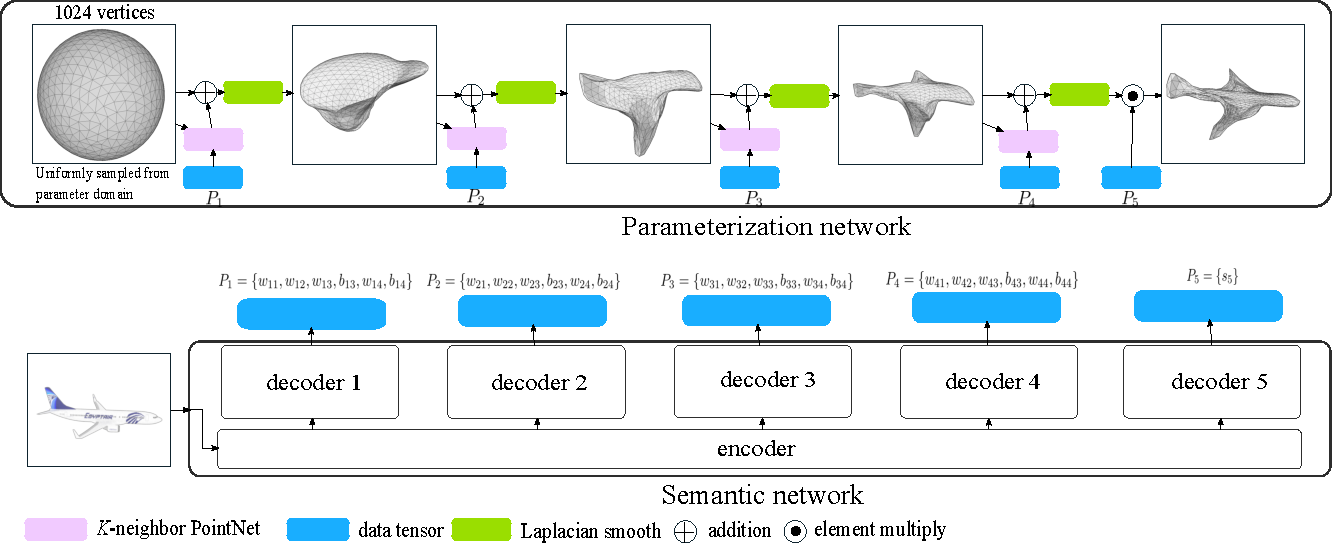
\includegraphics[width=\linewidth]{img/net/overview}
	\caption{The overview of the network: The proposed framework consists of two networks. One is the parameterization network that maps points sampled from parameter domain to target shape. The other is the semantic network that takes image as input and predict parameters for the parameterization network.}
	\label{fig:overview}
\end{figure*}

In summary, our contributions are
\begin{itemize}
	\item  Introduction of parameterization networks that enable mesh generation by representing the 3D shape as a spherical uniform distribution plus a learned/predicted mapping.
	\item  Exploring the idea that uses semantic network to predict parameters for parameterization network. Such structure relate input image to parameterization network.
	\item Though bijective is not ensured for the predicted mapping now, with the ability to integrate mesh based operation and losses, our framework push the neural network towards an actual \emph{parameterization prediction} network that would allow more mesh operation former studied in computer graphics to be integrated into neural networks.
\end{itemize}          

